% Document uses 12 pt font
% 1 in margins
% Contains a relative path for images

\documentclass [10pt]{article}

% page geometry 
\usepackage[margin=1in]{geometry}


% ----------  PACKAGES START ------------ %
% Math Packages
\usepackage{amsmath}
\usepackage{mathtools}

% Table cell color package and highlighting
\usepackage[table]{xcolor}
\usepackage{color,soul}

% VIC title package\
\usepackage[T1]{fontenc}

% default font package
%\usepackage{times}
\usepackage{helvet}
%\renewcommand{\familydefault}{\sfdefault}

% ---------- End Font Packages -------------- %

%\usepackage{listings}


\definecolor{dkgreen}{rgb}{0,0.6,0}
\definecolor{gray}{rgb}{0.5,0.5,0.5}
\definecolor{mauve}{rgb}{0.58,0,0.82}

\lstset{frame=tb,
  language=C++,
  aboveskip=3mm,
  belowskip=3mm,
  showstringspaces=false,
  columns=flexible,
  basicstyle={\small\ttfamily},
  numbers=none,
  numberstyle=\tiny\color{gray},
  keywordstyle=\color{blue},
  commentstyle=\color{dkgreen},
  stringstyle=\color{mauve},
  breaklines=true,
  breakatwhitespace=true,
  tabsize=3
}

% Title Packages
\usepackage{titlesec}
\usepackage{titletoc}

% Image Package
\usepackage{graphicx}

% Table Packages
\usepackage{longtable}
\usepackage{multirow}
\usepackage{multicol}
\usepackage{multirow}
\usepackage{array}
\renewcommand{\arraystretch}{1.2}% Spread rows out evenly in table
\setlength{\LTpre}{0.5pt} % Reduces white space around tables (top)
%\setlength{\LTpost}{0pt} % Reduces white space around tables (bottom)

% Color Packages
\usepackage{color}   
\definecolor{sectionC}{rgb}{0.95,0.52,.0}
\definecolor{subsectionC}{rgb}{1.0,.64,.26}
\definecolor{subsubsectionC}{rgb}{1.0,.87,.68}
\definecolor{tableCell}{rgb}{.98,.81,.69}


% List package
\usepackage{enumitem}
\setenumerate{itemsep=0pt, itemindent=0in,leftmargin=0.5in}


% Paragraph parameter

\setlength{\parindent}{0pt}


% ------------- Creates a linked Table of Contents  Start --------------- %
\usepackage{hyperref}
\hypersetup{
colorlinks=true, %set true if you want colored links
linktoc=all,     %set to all if you want both sections and subsections linked
linkcolor=black,}  %choose some color if you want links to stand out

% ------------- Creates a click-able Table of Contents  End--------------- %

% ---------- PACKAGES END ------------ %








% -------- SECTION AND SUBSECTION FORMATING START -------- % 
% starts the 
%\setcounter{section}{1}


\titleformat{\section} % Section
{\normalfont \fontsize{14}{14} \bfseries}{}{0em}{\colorsection}

% Makes a background color
\newcommand{\colorsection}[1]{%
  \colorbox{sectionC}{\parbox{\dimexpr\textwidth-1\fboxsep}{\color{white}\Large\thesection\ \hspace{1mm} #1}}}

% Makes a background color
\titleformat{\subsection} % Subsection
{\normalfont \fontsize{12}{12}  \bfseries}{}{0em}{\colorsubsection }

\newcommand{\colorsubsection}[1]{%
  \colorbox{subsectionC}{\parbox{\dimexpr \textwidth -1\fboxsep}{\large\thesubsection\ #1}}}


% Makes a background color
\titleformat{\subsubsection} % Subsubsection
{\normalfont \fontsize{12}{12} \bfseries}{}{0em}{\colorsubsubsection}

\newcommand{\colorsubsubsection}[1]{%
  \colorbox{subsubsectionC}{\parbox{\dimexpr\textwidth-1\fboxsep}{\thesubsubsection\ #1}}}

% -------- SECTION AND SUBSECTION FORMATING END -------- % 
\usepackage{lipsum}


% -----  IMAGE PATH START -----%
% Relative Image Path
\graphicspath {figures/}
% -----  IMAGE PATH END -----%

% ------ PARAGRAPH FORMAT START ----%
%\setlength{\parskip}{.2em}% Sets the space between new paragraph items 
\setlength{\parindent}{0em} % paragraph indent
% ------ PARAGRAPH FORMAT END ----%




%------------------------------TOC FORMAT START --------------------------------%
\usepackage{tocloft}



% Section indentations
\cftsetindents{section}{0em}{1.5em}
\cftsetindents{subsection}{1em}{2em}
\cftsetindents{subsubsection}{2em}{3em}

% Toc title size
\renewcommand\cfttoctitlefont{\Large\bfseries}
\renewcommand*\contentsname{Table of Contents}

\newcommand{\carSpeed}{1.4\ m/s}
\newcommand{\intersectionLength}{0.6\ m}


% Removes bold headings from toc
%\renewcommand{\cftsecfont}{\normalfont}

% Removes bold heading page numbers from toc
\renewcommand{\cftsecpagefont}{\normalfont}

% add dots after headings
%\renewcommand{\cftsecleader}{\cftdotfill{\cftdotsep}} 


% number of section headings we want to see in toc
\setcounter{tocdepth}{2}

% Spaceing before headings in toc
\setlength{\cftbeforesecskip}{6pt}

% ------------------------------TOC FORMAT END --------------------------------%



% ------------------- START HEADER AND FOOTER ---------------------------%
\usepackage{fancyhdr}

% Helps with the n of total n pages
\usepackage{lastpage}

\pagestyle{fancy}

% Header
\lhead{Component Design}
\rhead{Revision: 0}
\fancyhead[LE,CO]{Group 9: LazyBots}

% Removes line under the header 
\renewcommand{\headrulewidth}{0pt}
\setlength{\headsep}{.2in}

% Footer 

% Set the right side of the footer to be the page number
\fancyfoot[R]{Page \textbf{\thepage}\ of \textbf{\pageref{LastPage}}}
\fancyfoot[C]{}

% ------------------- END HEADER AND FOOTER ---------------------------%






% -------------- DOCUMENT START ---------------%
\begin{document}

% --------- TITLE PAGE START ------- %
\begin {center} 

\thispagestyle{empty}
\vspace*{5cm}

% Logo Insertion
\begin {figure}[h!]
\centering
\hspace{-10mm}
\includegraphics [scale = .3, trim={.4cm 0 .8cm 0},clip] {figures/alfred.png}
\end {figure}

\Huge{LazyBots}

\vspace{1 cm}
{\Large\textbf{\textsc{McMaster University}}\\}  \vspace {1cm}
{\Large Draft Component Design\\ \vspace {0.4 cm} SE 4GA6 \& TRON 4TB6}  \vspace {1cm}

{\large \textsc{Group 9} \\} \vspace{1cm}



\begin{tabular}{ l c  l}
Karim Guirguis & & 001307668 \\
David Hemms & & 001309228 \\
Marko Laban & & 001300989 \\
Curtis Milo & & 001305877 \\
Keyur Patel & & 001311559 \\
Alexandra Rahman & & 001305735
\end{tabular}


\end{center}


% --------- TITLE PAGE END------- %

\pagebreak

% Inserting table of contents and table of figures 

\tableofcontents
\listoftables
\listoffigures



\pagebreak

% -----------  REVISION HISTORY START ----------- %

%\section*{Revisions}
\thispagestyle{empty}
\section{Revisions}
\begin{longtable}{| p{.2\textwidth } | p{.23\textwidth } | p{.23\textwidth } | p{.23\textwidth } |} \caption{VIC Table of Revisions}  \\

% ------------------------------------------------------- Date ------------------------------------------------------- %
\hline 
\centering \textbf{Date} & 
\multicolumn{1}{c}{\textbf {Revision Number}} &
\multicolumn{1}{|c}{\textbf {Authors}} & 
\multicolumn{1}{|c|}{\textbf {Comments}} \\ \hline

% ------------------------------------------------------- Revision Number -------------------------------------------------------
\multirow{4}{*}{\centering November 24\textsuperscript{th}, 2017}  & 
\multirow{4}{*}{Revision 0}& 
		{Karim Guirguis \newline
		David Hemms \newline
		Marko Laban \newline
		Curtis Milo \newline
		Keyur Patel \newline
		Alexandra Rahman}
 &
 
% ------------------------------------------------------- Comments -------------------------------------------------------
\multirow{4}{*}{-} \\ 
\hline 

\end{longtable}



\pagebreak

%---------------------------- PROJECT DRIVERS ------------------------%
% heading in document

% -------------- START INTRODUCTION ---------------- %


\section {Manager System}


\subsection{Purpose}
The following will describe the component software design associated with Manager System. This will be carried out within web based tools to allow managment to access there information Anywhere

\subsection{Scope}

The scope of this section is associated with any front end user interfaces that the managment staff will use. This includes the MIS/MID and uses relation in regards to the Map Making Page, the Error Viewing page and the Login System. 

\subsection{Module Decomposition}

\textbf{Manager Login Page}: Given the login credentials, will authenticate administrator of the system with the server. Secrets include how it goes about verifying with the server if the credentials are valid.
\textbf{Manager Station Map Software Page}: Will allow administrator to create or modify the map of the area where Alfred will deliver drinks. This map will then be sent and stored on the server. The secrets of this module includes how the mapping system will translate user input into the map file
\textbf{Manager Station Request Software Page}: Will allow administrator to execute commands for Alfred, as well as view incoming error codes from Alfred. Secrets include how the errors are decoded from the server.

\subsection{Uses Relation}
\begin{figure} [h!]
	\centering
	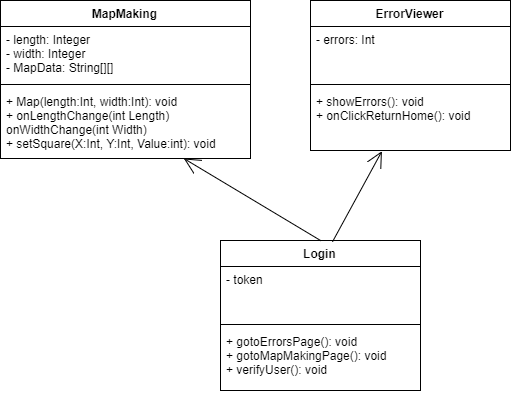
\includegraphics [scale = 0.4] {figures/Manager_UsesDiagram.png}
	\caption{Alfred Uses Relation Diagram}
\end{figure}

\subsection{MIS}

\subsubsection{Login Page}
\textbf{Uses}
\begin{itemize}
	\item MapMaking (WebPage)
	\item ErrorViewer (WebPage)
\end{itemize}



\textbf{Public Functions}

\textbf{gotoErrorsPage(): void}
Navigates to the page associated with showing the Managers page for Errors with Alfred.

\textbf{gotoMapMakingPage(): void}
Navigates to the page associated with showing the Managers page for creating a resturant Map.

\textbf{verifyUser(): void}
Determines if the information that the user put into the form on the webpage is correct.


\subsubsection{MapMaking Page}
\textbf{Uses}
None

\textbf{Public Functions}

\textbf{ Map(length:Int, width:Int): void}
Constructor to object for page load

\textbf{onLengthChange(int Length)}
Sets the length of the map when the user changes it in the form.

\textbf{onWidthChange(int Width)}
Sets the width of the map when the user changes it in the form.

\textbf{setSquare(X:Int, Y:Int, value:Int): void}
Sets the value of the square based on its X,Y position when there is an on click event.

\subsubsection{ErrorViewer Page}
\textbf{Uses}
None

\textbf{Public Functions}

\textbf{ showErrors(): void}
Shows the Errors Associated to Alfred.
\textbf{onClickReturnHome()}
Signals the Robot to return home.

\subsection{MID}

\subsubsection{Login Page}
\textbf{Uses}
\begin{itemize}
	\item MapMaking (WebPage)
	\item ErrorViewer (WebPage)
\end{itemize}


\textbf{Internal Variables}

\textbf{token: String} - Token for a session with the server.


\textbf{Functions}

\textbf{public gotoErrorsPage(): void}
Navigates to the page associated with showing the Managers page for Errors with Alfred.

\textbf{public gotoMapMakingPage(): void}
Navigates to the page associated with showing the Managers page for creating a resturant Map.

\textbf{public verifyUser(): void}
Determines if the information that the user put into the form on the webpage is correct.


\subsubsection{MapMaking Page}
\textbf{Uses}
None

\textbf{Internal Variables}

\textbf{length: Integer} - Length of the Map

\textbf{width: Integer} - Width of the Map

\textbf{MapData: String[][]}- Storage of the map values

\textbf{Public Functions}

\textbf{public Map(length:Int, width:Int): void}

Constructor to object for page load

\textbf{public onLengthChange(int Length)}

Sets the length of the map when the user changes it in the form.

\textbf{public onWidthChange(int Width)}

Sets the width of the map when the user changes it in the form.

\textbf{setSquare(X:Int, Y:Int, value:Int): void}

Sets the value of the square based on its X,Y position when there is an on click event. The Values corresponds to: 
 
\begin{itemize}
	\item 0: Free to move
	\item 1: Path is blocked
	\item 2: Table
	\item 3: Base
\end{itemize}

\subsubsection{ErrorViewer Page}
\textbf{Uses}
None

\textbf{Public Functions}

\textbf{ showErrors(): void}
Shows the Errors Associated to Alfred. where the Errors are in the following format
\begin{itemize}
	\item LowLiquid: 0x00000001
	\item LeakingTank: 0x00000010
	\item LowBattery: 0x00000100
	\item NoMovement: 0x00001000
\end{itemize}

\textbf{onClickReturnHome()}
Signals the Robot to return home.

\section {Alfred System}


\subsection{Purpose}
The following will describe the component software, mechanical and electrical design associated with Alfred's Manager System, Alfred's Drivetrain and Alfred's Image Processing system. These three systems will be ran on the Raspberry Pi. 

\subsection{Scope}

The scope of this section is associated with Alfred's Manager System, Alfred's Drivetrain and Alfred's Image Processing system. The software documentation will provide the MIS and MID, uses relations to describe how the system will be designed to preform its function of being able to drive to a specific location. The mechanical and electrical design will focus on the aspects to provide motion and navigation.


\subsection{Module Decomposition}

\textbf{Alfred Manager Module}: Endpoint for communication with Alfred. Will manage communication with server, as well as send any errors that Alfred is experiencing. Secrets include Parsing of messages from the server and the pumping system. 
\textbf{Alfred Drive Train Module}: Responsible for driving and managing the motors based on desired route. Will also be sending errors preventing movement to Alfred Manager Module. Secrets include how the robot will preform navigation based on the map, how the robot will control and drive the robot and the inputs from the image processing module.
\textbf{Image Processing Module}: Will detect any obstacles in the way as well as locate incoming nodes. Will communicate with Alfred Drive Train Module, to determine whether any required action based on results. Secretes include how the image processing will be carried out

\subsection{Uses Relation}
\begin{figure} [h!]
	\centering
	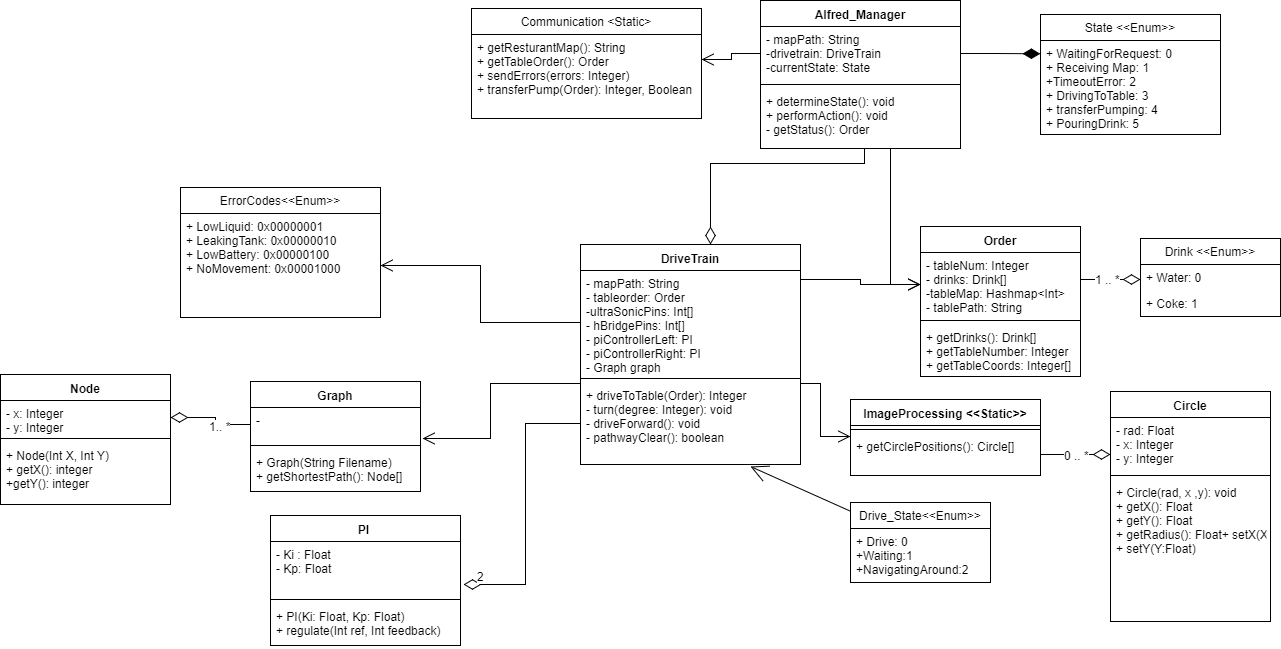
\includegraphics [scale = 0.4] {figures/Alfred_UsesDiagram.png}
	\caption{Alfred Uses Relation Diagram}
\end{figure}


\subsection{MIS}

\subsubsection{Alfred Manager Class}

\textbf{Uses}
\begin{itemize}
	\item Communication (Static Class)
	\item State (Enum)
	\item Drivetrain (Class)
	\item Order (Class)
\end{itemize}



\textbf{Public Functions}

\textbf{determineState(): void}

Determines the overall state of Alfred based on the inputs to Alfred.

\textbf{performAction(): void}

Will preform the desired state based on the state of Alfred.

\subsubsection{Order Class}
\textbf{Uses}
\begin{itemize}
	\item Drink (Enum)
\end{itemize}


\textbf{Public Functions}

\textbf{getDrinks()}

Drink[] - Returns the list of drinks

\textbf{getTableNumber}

 Integer - Returns the table number reference

\textbf{getTableCoords}

 Integer[] - Returns the coordinates to the table

\subsubsection{Drivetrain Class}
\textbf{Uses}
\begin{itemize}
	\item Order (Class)
	\item ImageProcessing (Class)
	\item Drive\_State (Enum)
	\item ErrorCodes (Enum)
	\item Circle (Class)
	\item Graph (Class)
	\item Node (Class)
	\item PI (Class)
\end{itemize}

\textbf{Public Functions}
\textbf{driveToTable(Order): Integer}
This function will preform the driving operation in order to navigate towards the specific table.

\subsubsection{Communication Static Class}
\textbf{Uses}

None 

\textbf{Public Functions}

\textbf{getResturantMap(): String}

Retrieves and stores the map to be used for navigation. Returns the path of the map 

\textbf{getTableOrder(): Order}

Retrieves and returns the Table's Order.

\textbf{sendErrors(errors: Integer)}

Sends an integer with the described set of integers. 

\textbf{transferPump(Order): Integer}

Preforms communication with the pumping system. Sends the Order data and receives the errors from the pumping system and if it complete.

\subsubsection{Graph Class}
\textbf{Uses}
\begin{itemize}
	\item Node (Class)
\end{itemize}

\textbf{Public Functions}

\textbf{Graph(String Filename)}

Constructor to create a graph object. Builds the graph based on the path to the map

\textbf{getShortestPath(): Node[]}

Returns a list of nodes that describes the shortest way to get to the destination. 


\subsubsection{Node Class}
\textbf{Uses}
None 

\textbf{Public Functions}

\textbf{Node(Int X, Int Y)}

Constructor to the node class, takes in the position of the point along the X Y plane.

\textbf{getX(): integer}


Returns the x coordinate of the node

\textbf{getY(): integer}

Returns the y coordinate of the node

\subsubsection{PI Class}
\textbf{Uses}
None 

\textbf{Public Functions}

\textbf{PI(Ki: Float, Kp: Float)}

Constructor for the PI controller object taking in the Ki and Kp terms

\textbf{regulate(Int ref, Int feedback)}

Based on the reference to control to and the feedback, will determine the value to set the outputs too.

\subsubsection{Imaging Processing Static Class}
\textbf{Uses}
\begin{itemize}
	\item Circle (Class)
\end{itemize}

\textbf{Public Functions}

\textbf{getCirclePositions(): Circle[]}

Gives a list of circles that were within the view of the camera

\subsubsection{Circle Class}

\textbf{Uses}
None

\textbf{Public Functions}

\textbf{Circle(radius, x, y)}

Constructor of the circle class, takes in initial radius, x and y values

\textbf{getX(): Float}

Gives the X position of the circle relative to the image

\textbf{getY(): Float}

Gives the Y position of the circle relative to the image

\textbf{getRadius(): Float}

Gives the radius of the circle

\textbf{setX(X:Float)}

Sets the X position of the circle.

\textbf{setY(Y:Float)}

Sets the Y position of the circle.

\textbf{setRadius(rad : Float)}

Sets the radius of the circle

\subsection{MID}

\subsubsection{Alfred Manager Class}

\textbf{Uses}
\begin{itemize}
	\item Communication (Static Class)
	\item State (Enum)
	\item Drivetrain (Class)
	\item Order (Class)
\end{itemize}


\textbf{Internal Variables}

\textbf{mapPath: String} - The absolute path to the map directory

\textbf{drivetrain: DriveTrain} - An object encapsulates information in regards to the drivetrain

\textbf{currentState: State} - Holds the information in regards to which action will be preformed by Alfred


\textbf{Functions}

\textbf{public determineState(): void}

Determines the overall state of Alfred based on the inputs to Alfred based on the following tabular expression:
\begin{figure} [h!]
	\centering
	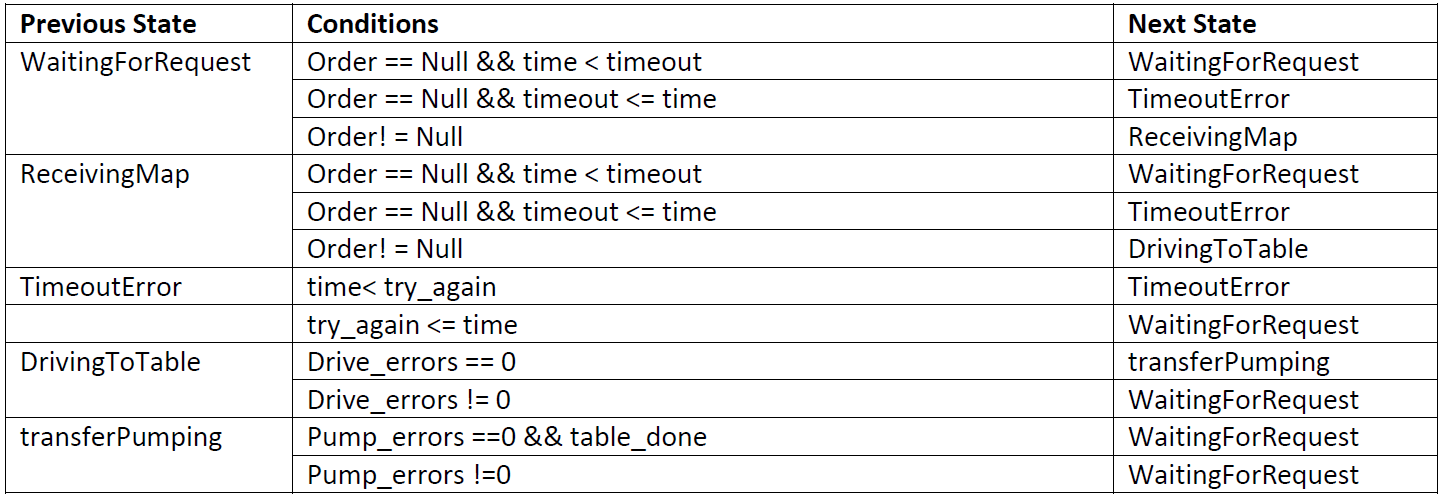
\includegraphics [scale = 0.4] {figures/AlfredSystem_DetermineState.png}
\end{figure}


\textbf{public performAction(): void}

Will preform the desired state based on the state of Alfred based on the following table:
\begin{figure} [h!]
	\centering
	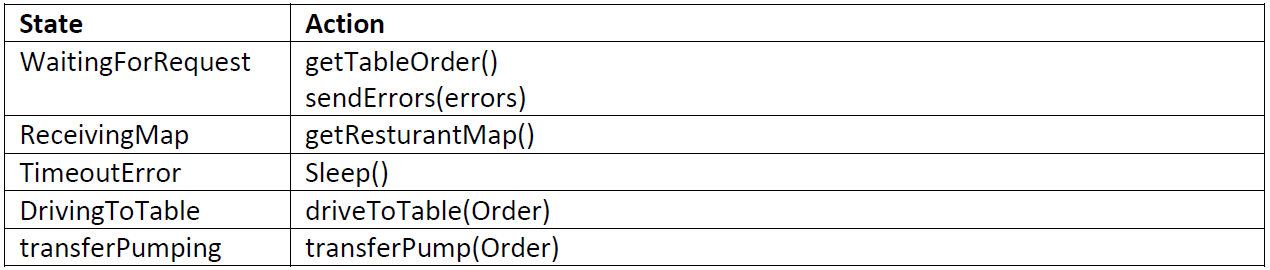
\includegraphics [scale = 0.4] {figures/AlfredSystem_PerformAction.png}
\end{figure}
\subsubsection{Order Class}
\textbf{Uses}
\begin{itemize}
	\item Drink (Enum)
\end{itemize}


\textbf{Internal Variables}

\textbf{tableNum: Integer} - the reference to the table

\textbf{drinks: Drink[]} - List of drinks for the user's table

\textbf{tableMap: Hashmap<Int>} -  Map that takes in a table reference number and returns its X,Y Coord

\textbf{tablePath: String} - gives the path of the table for the hashmap 

\textbf{Functions}

\textbf{public getDrinks(): Drink[]}

Returns the list of drinks

\textbf{public getTableNumber: Integer}

Returns the table number reference

\textbf{public getTableCoords: Integer[]}

Returns the coordinates to the table from the Hashmap of table numbers

\subsubsection{Drivetrain Class}
\textbf{Uses}
\begin{itemize}
	\item Order (Class)
	\item ImageProcessing (Class)
	\item Drive\_State (Enum)
	\item ErrorCodes (Enum)
	\item Circle (Class)
	\item Graph (Class)
	\item Node (Class)
	\item PI (Class)
\end{itemize}


\textbf{Internal Variables}
\textbf{mapPath: String} - The absolute path to the map directory

\textbf{tableorder: Order} - The order from the next table.

\textbf{ultraSonicPins: Int[]} - The pins dedicated for the ultrasonic sensors

\textbf{hBridgePins: Int[]} - The pins dedicated for the H-bridge

\textbf{graph: Graph} - Object to the graph object to find the shortest path

\textbf{piControllerLeft: PI} - Object used for PI control for the left side of the drivetrain

\textbf{piControllerRight: PI} - Object used for PI control for the left side of the drivetrain

\textbf{Functions}

\textbf{public driveToTable(Order): Integer}

This function will preform the driving operation in order to navigate towards the specific table.

\textbf{private turn(degree: Integer): void}

This function will turn relative to its current position the amount desired within the argument. The robot will use the references of the circles to help with alignment by knowing that every node is 90 degrees from one another.

\textbf{private driveForward(void): void}

This function will control the robot to move forward provided: $ \forall front ultrasonic sensors: d_{ultrasonic} > d_{min} $. This motion will use the PI regulators to provide motion at human speed and will continue until a the next circle is within the middle of the camera.

\textbf{private pathwayClear (void): boolean}

This function will determine if robot to move forward provided: $ \forall front ultrasonic sensors: d_{ultrasonic} > d_{min} $. 

\subsubsection{Communication Static Class}
\textbf{Uses}
None 
\textbf{Internal Variables}

None 

\textbf{Functions}

\textbf{getResturantMap(): String}

Retrieves the map file based off of an FTP protocol and stores the map to be used for navigation. Returns the path of the map.

\textbf{getTableOrder(): Order}

Retrieves and returns the Table's Order.

\textbf{sendErrors(errors: Integer)}

 Sends an integer with the described set of integers. 
 
\textbf{transferPump(Order): Integer}

 Performs communication with the pumping system using UART communication. The first 32 bits are the error code of the pumping system and the last bit is the status of the pumping system. Sends the Order data and receives the errors from the pumping system.

\subsubsection{Graph Class}
\textbf{Uses}
\begin{itemize}
	\item Node (Class)
\end{itemize}

\textbf{Internal Variables}
None 

\textbf{Functions}

\textbf{Graph(String Filename)}

Constructor to create a graph object. Builds the graph based on the path to the map

\textbf{getShortestPath(): Node[]}

Returns a list of nodes that describes the shortest way to get to the destination.  The shortest path will be preformed using the map and Dijkstra's algorithm.


\subsubsection{Node Class}
\textbf{Uses}
None 

\textbf{Public Functions}

\textbf{Node(Int X, Int Y)}

Constructor to the node class, takes in the position of the point along the X Y plane.

\textbf{getX(): integer}

Returns the x coordinate of the node.

\textbf{getY(): integer}

Returns the y coordinate of the node.

\textbf{Internal Variables}

\textbf{x: Integer} - The x coordinate of the node

\textbf{y: Integer} - The y coordinate of the node

\textbf{Functions}

\textbf{public Node(Int X, Int Y)}

Constructor to the node class, takes in the position of the point along the X Y plane.

\textbf{public getX(): integer}

Returns the x coordinate of the node

\textbf{public getY(): integer}

Returns the y coordinate of the node


\subsubsection{PI Class}
\textbf{Uses}
None 
\textbf{Internal Variables}
\textbf{Ki: Float} - Integral temp for the PI controller
\textbf{Kp: Float} - The y coordinate of the node.

\textbf{Functions}

\textbf{public PI(Ki: Float, Kp: Float)}

Constructor for the PI controller object taking in the Ki and Kp terms

\textbf{public regulate(Int ref, Int feedback)}

Based on the reference to control to and the feedback, will determine the value to set the outputs too. Determines the output based along the following formula: $ out = Kp*error+Ki*\int_{0}^{t}(error)dt$. Note that the derivative term is not used due to the error associated with derivatives within computing systems.


\subsubsection{Imaging Processing Static Class}
\textbf{Uses}
\begin{itemize}
	\item Circle (Class)
	\item Open CV (External Library)
\end{itemize}


\textbf{Internal Variables}
None

\textbf{Functions}

\textbf{Public getCirclePositions(): Circle[]}

Gives a list of circles that were within the view of the camera. Open CV returns a list of objects which can then be checked to see if they are black circles.

\subsubsection{Circle Class}

\textbf{Uses}
None
\textbf{Internal Variables}

\textbf{rad: Float} - The radius of the circle

\textbf{x: Integer} - The X position of the circle relative to the image

\textbf{y: Integer} - The Y position of the circle relative to the image 

\textbf{Functions}

\textbf{Circle(radius, x, y)}

Constructor of the circle class, takes in initial radius, x and y values

\textbf{getX(): Float}

Gives the X position of the circle relative to the image

\textbf{getY(): Float}

Gives the Y position of the circle relative to the image

\textbf{getRadius(): Float}

Gives the radius of the circle

\textbf{setX(X:Float)}

Sets the X position of the circle.

\textbf{setY(Y:Float)}

Sets the Y position of the circle.

\textbf{setRadius(rad : Float)}

Sets the radius of the circle.


\section {Pumping System}

\subsection{Purpose}
The following will describe the component software, mechanical and electrical design associated with Alfred's Pumping System, Alfred's Drivetrain and Alfred's Image Processing system. This system will be ran on the Arduino Mega.
\subsection{Scope}

The scope of this section is associated with Alfred's Pumping System. The software documentation will provide the MIS and MID, uses relations to describe how the system will be designed to preform its function of being able to communicate to the raspberry pi and pump drinks. The mechanical and electrical design will focus on the different pumps/sensors that will be associated with the pumping system.


\subsection{Module Decomposition}

\textbf{Alfred Pumping Module}: Will control pumping system in regards of when to pour, how long and rate of dispensing. Will communicate to the raspberry pi errors pertaining to the pump or container to Alfred Manager Module. secrets include how the system preforms the dispensing of drinks and determination of errors.

\subsection{Uses Relation}
\begin{figure} [h!]
	\centering
	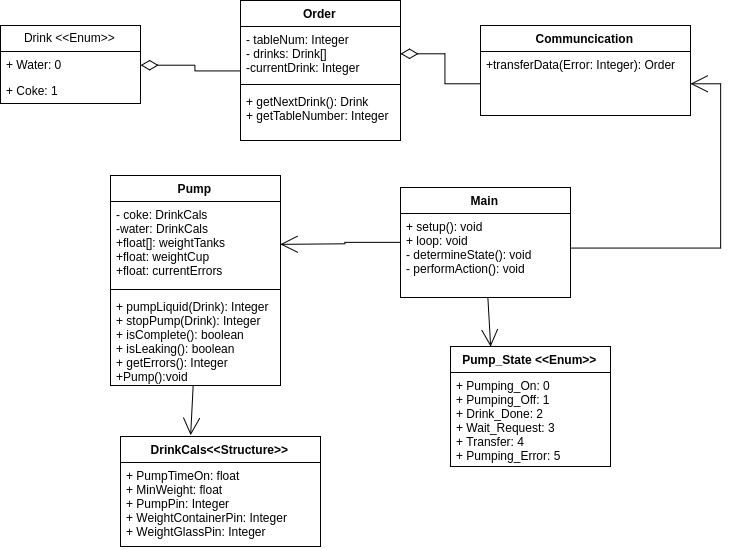
\includegraphics [scale = 0.4] {figures/Pumping_UsesDiagram.png}
	\caption{Uses Relation Diagram for the pumping system}
\end{figure}


\subsection{MIS}

\subsubsection{Main Class}

\textbf{Uses}
\begin{itemize}
	\item Order (Class)
	\item Drink (Enum)
	\item Pump (Class)
	\item Pump\_State (Enum)
	\item Communication (Class)
\end{itemize}

\textbf{Internal Variables}
None

\textbf{Functions}

\textbf{public setup(): void}

Setup function for Arduino that initializes the pins that will be used 

\textbf{publicloop(): void}

Main loop that will preform the main logic of the pumping system

\textbf{public determineState(): void}

Based on the previous state of the pumping machine will look at factors such as weight of the liquid, need for communication and errors to determine the next state.

\textbf{public performAction(): void}

Based on the state of the device it will:
\begin{itemize}
	
	\item Pumping\_On: Turn on the voltage for the pump
	\item Pumping\_Off: Turn off the voltage for the pump
	
	\item Wait\_Request: Will Sleep for a specific amount of time before checking again
	\item Transfer: Preform transferring via UART
	\item Pumping\_Error: Perform No Action, and ensure all pumping devices are off
\end{itemize}

\subsubsection{Class Pump}

\textbf{Uses}

\begin{itemize}
	\item DrinkCals
\end{itemize}


\textbf{public Functions}

\textbf{Pump():void}

Initializes the values of the pumping module.

\textbf{pumpLiquid(Drink): Integer}

Turns on the pump for the specific drink type.

\textbf{stopPump(Drink): Integer}

Turns off the pump for the specific drink type.

\textbf{isComplete(): Boolean}

Determines if the drink has been completely filled or not based.

\textbf{isLeaking(): Boolean}

Determines if the containers are losing fluid when there is no pumping.

\textbf{isSafeTempature()}

Determines if the containers are still storing the liquids are at a safe temperature.

\subsubsection{Communication Class}

\textbf{Uses}

\begin{itemize}
	\item DrinkCals
\end{itemize}

\textbf{Internal Values}
None

\textbf{Functions}

\textbf{transferData(Integer): Order}

Communication performed used  where Orders are received and errors are transferred with the Manager system.


\subsection{MID}

\subsubsection{Main Class}

\textbf{Uses}
\begin{itemize}
	\item Order (Class)
	\item Drink (Enum)
	\item Pump (Class)
	\item Pump\_State (Enum)
	\item Communication (Class)
\end{itemize}

\textbf{Internal Variables}

 None

\textbf{Functions}

\textbf{public setup(): void}

Setup function for Arduino that initializes the pins that will be used 

\textbf{public loop(): void}

Main loop that will preform the main logic of the pumping system

\textbf{public determineState(): void}

Based on the previous state of the pumping machine will look at factors such as weight of the liquid, need for communication and errors to determine the next state. Which state is summarized in the following table:
\begin{figure} [h!]
	\centering
	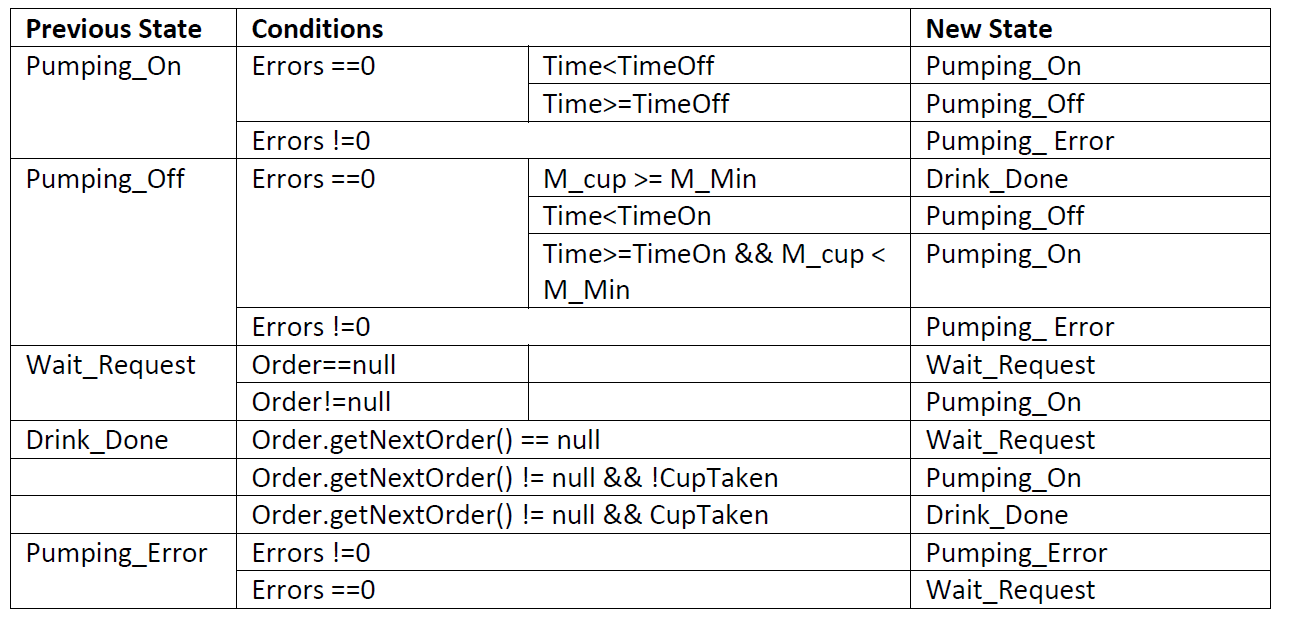
\includegraphics [scale = 0.4] {figures/Pumping_DetermineState.png}
\end{figure}

\textbf{public performAction(): void}

Based on the state of the the pumping system, will preform the following actions:
\begin{figure} [h!]
	\centering
	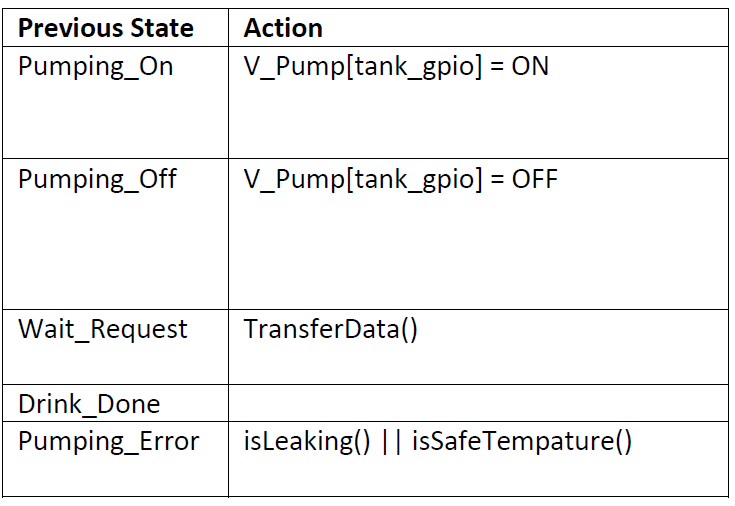
\includegraphics [scale = 0.4] {figures/Pumping_PerformActions.png}
\end{figure}


\subsubsection{Class Pump}

\textbf{Uses}

\begin{itemize}
	\item DrinkCals
\end{itemize}

\textbf{Internal Values}

\textbf{DrinkCals coke}: Structure holding the calibrations related to Coke products

\textbf{DrinkCals water}: Structure holding the calibrations related to Water

\textbf{Functions}

\textbf{public Pump():void}

Initializes the values of the pumping module.

\textbf{public pumpLiquid(Drink): Integer}

Turns on the pump for the specific drink type.

\textbf{public stopPump(Drink): Integer}

Turns off the pump for the specific drink type.

\textbf{public isComplete(): Boolean}

Determines if the drink has been completely filled or not based on the following equation:
$Filled := M_min < M_cup$

\textbf{public isLeaking(): Boolean}

Determines if the containers are losing fluid when there is no pumping based on the following equation:
$Leaking := [M_minleak < (M_container1 - M_container_prev1) \wedge Pin7 ==0] \vee [M_minleak < (M_container2 - M_container_prev2) \wedge Pin8 ==0] $

\textbf{public isSafeTempature()}

Determines if the containers are still storing the liquids at a temperature greater then the minimum temperature for the liquids based off of the following equations.
$OverTempature := (T_container1 < T_min) \vee (T_container2 < T_min)$ 


\subsubsection{Communication Class}

\textbf{Uses}

\begin{itemize}
	\item DrinkCals
\end{itemize}

\textbf{Internal Values}
 None

\textbf{Functions}

\textbf{transferData(Integer): Order}

Communication performed used using UART where Orders are received and errors are transferred. The first 32 bits will be the errors associated with the pumping system and the last bit will be if the robot is done.



\section {Server}
\subsection{Purpose}
The following will describe the component software design associated with the server. This system will be run on an external RHEL server.

\subsection{Scope}
The scope of this section is associated with the REST API server that will be responsible for the communication within the system. The software documentation will provide the MIS and MID, uses relations to describe how the system will be designed to perform its function of being able to route communication between difference modules in the system.

\subsection{Module Decomposition}
\textbf{Serer Module}: Will have different REST API endpoints available to be able to "perform actions" in different parts of the system, as well as route data.

\subsection{Uses Relation}
\begin{figure} [h!]
	\centering
	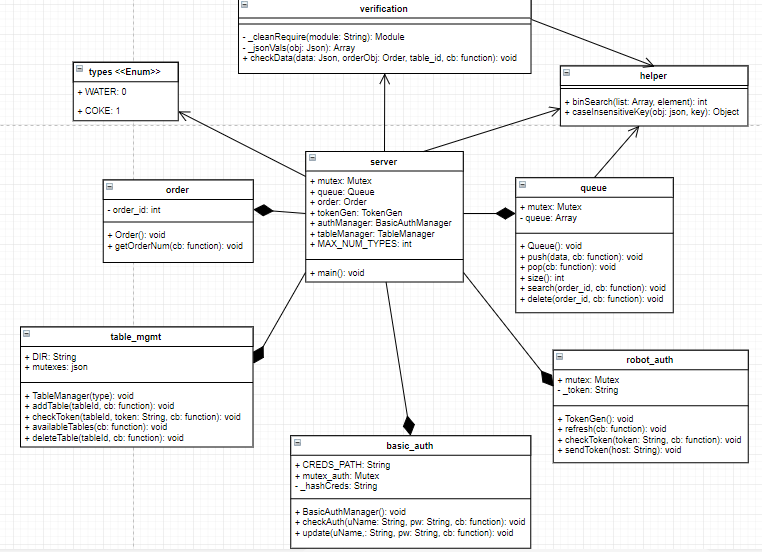
\includegraphics [scale = 0.4] {figures/server_class_diagram.PNG}
	\caption{Alfred Uses Relation Diagram}
\end{figure}

\subsection{MIS}
\subsubsection{server}
\textbf{Uses}
\begin{itemize}
	\item order (Class)
	\item types (Enum)
	\item verification (Class)
	\item helper (Class)
	\item queue (Class)
	\item robot\_auth (Class)
	\item basic\_auth (Class)
	\item table\_mgmt (Class)
	\item http (External Class)
	\item url (External Class)
	\item fs (External Class)
	\item locks (External Class)
\end{itemize}

\textbf{Public Functions}
\textbf{main(): void}
Running the server, intercepting REST API requests and taking required action.

\subsubsection{queue}
\textbf{Uses}
\begin{itemize}
	\item locks (External Class)
	\item helper (Class)
\end{itemize}

\textbf{Public Functions}
\textbf{Queue(): void}
Constructor function that creates a new empty queue.

\textbf{push(data, cb): void}
Push new order information into the queue and callback function with the place in line.

\textbf{pop(cb): void}
Pops the first element from the queue.

\textbf{size(): int}
calls the callback function with the current size of the queue.

\textbf{search(order\_id, cb): void}
Searches the queue and calls callback function with the place in line for the order specified by the order\_id.

\textbf{delete(order\_id, cb): void}
Searches the queue for order identified by given order\_id and removes it from the queue.

\subsubsection{helper}
\textbf{Uses}
None

\textbf{Public Functions}
\textbf{binSearch(list, element): int}
Binary search algorithm to find an element and return its position. If element not found, returns -1.

\textbf{caseInsensitiveKey(obj, key): obj[i]}
Extracts information from a JSON object for a given key. Comparison between the key and the JSON object's keys are case insensitive.

\subsubsection{basic\_auth}
\textbf{Uses}
\begin{itemize}
	\item fs (External Class)
	\item locks (External Class)
	\item util (External Class)
	\item crypto (External Class)
\end{itemize}

\textbf{Public Functions}
\textbf{BasicAuthManager(): void}
Constructor function to create the object.

\textbf{checkAuth(uName, pw, cb): void}
Will check the validity of the username and password given as parameters, and will call the callback function with a boolean of whether username/password combination is valid.

\textbf{update(uName, pw, cb): void}
Will update the stored username and password combination, with the given ones.

\subsubsection{robot\_auth}
\textbf{Uses}
\begin{itemize}
	\item locks (External Class)
	\item rand-token (External Class)
	\item unirest (External Class)
\end{itemize}

\textbf{Public Functions}
\textbf{TokenGen(): void}
Constructor function to create the object with new token.

\textbf{refresh(cb): void}
Updates current token.

\textbf{checkToken(token, cb): void}
Check that the given token in the parameters matches the token stored in the object, and calls the callback function with boolean result.

\textbf{sendToken(host): void}
Will send current token to the 'host' given in the parameters.

\subsubsection{verification}
\textbf{Uses}
\begin{itemize}
	\item helper (Class)
	\item types (Enum)
\end{itemize}

\textbf{Public Functions}
\textbf{checkData(data, orderObj, table\_id, cb): void}
Verify that the order information in the HTTP request has all necessary information and is in the correct format. Information required includes drink types, sizes, and quantities. Then calls callback function with error, if one exists.

\subsubsection{table\_mgmt}
\textbf{Uses}
\begin{itemize}
	\item locks (External Class)
	\item rand-token (External Class)
	\item fs (External Class)
	\item crypto (External Class)
\end{itemize}

\textbf{Public Functions}
\textbf{TableManager(): void}
Constructor function that reads all currently listed tables from the tables filesystem and creates a mutex for each.

\textbf{addTable(tableId, cb): void}
Register a new table with the filesystem and generate an authentication token for that table to be used with server communication, then calls the callback function with the token.

\textbf{checkToken(tableId, token, cb): void}
Verify that an inputted token is correct for the table, and calls callback function with boolean result.

\textbf{availableTables(cb): void}
Search the filesystem to find all tables currently registered, and call callback function with list of all tables.

\textbf{deleteTable(tableId, cb): void}
Remove a table from the filesystem.

\subsubsection{order}
\textbf{Uses}
\begin{itemize}
	\item locks (External Class)
\end{itemize}

\textbf{Public Functions}
\textbf{Order(): void}
Constructor function that creates a new Order object, with order\_id == 0.

\textbf{getOrderNum(cb): void}
Call the callback function with the next order\_id and increment the counter.

\subsection{MID}
\subsubsection{server}
\textbf{Uses}
\begin{itemize}
	\item order (Class)
	\item types (Enum)
	\item verification (Class)
	\item helper (Class)
	\item queue (Class)
	\item robot\_auth (Class)
	\item basic\_auth (Class)
	\item table\_mgmt (Class)
	\item http (External Class)
	\item url (External Class)
	\item fs (External Class)
	\item locks (External Class)
\end{itemize}

\textbf{Internal Values}
\begin{itemize}
	\item Mutex mutex: Mutex to synchronize requests updating value of 'types.json' in the filesystem.
	\item Queue queue: A FIFO queue where orders are stored.
	\item Order order: Object to keep track of order ID's.
	\item TokenGen tokenGen: A token generator and manager for the robot token for authentication.
	\item BasicAuthManager authManager: Object responsible for authenticating administrator.
	\item TableManager tableManager: Object responsible for authenticating each table.
	\item final int MAX\_NUM\_TYPES: Variable storing maximum number of types of drinks that the robot can hold.
\end{itemize}

\textbf{Functions}
\textbf{main(): void}

\begin{center}
	\begin{tabular}{ |c|c|c| } 
		\hline
		GET & POST & DELETE \\ 
		placeinline & placeorder & cancelorder \\ 
		nextorder & gentoken & drinks \\ 
		checktoken & updatecreds & tables \\ 
		drinks & returntobase &  \\ 
		sizes & login &  \\ 
		numoftanks & errors &  \\ 
		& drinks &  \\ 
		& tables &  \\ 
		\hline
	\end{tabular}
\end{center}

\textbf{Placeinline}
Call checkToken for table authentication
If passed, search queue for order\_id
res.write(placeInLine.toString());
\textbf{Placeorder}
Call checkToken for table authentication
If passed, parse the body of the request
Verify that all data is correct
If correct, push order to queue
\textbf{cancelOrder}
Call checkToken for robot authentication
If passed, delete order from queue for specific order\_id
\textbf{Nextorder}
Call checkToken for robot authentication
If passed, call queue’s pop function
res.write(placeInLine.toString());
\textbf{Gentoken}
Call token refresh function
Send token to robot host
\textbf{Checktoken}
Call checkToken for robot authentication
res.write(JSON.stringify(resp\_auth));
\textbf{Updatecreds}
Call checkAuth for admin authentication
If passed, parse body of request
Call authManager update function to update new user/password combination
\textbf{Login}
Call checkAuth for admin authentication
res.writeHead(200, 'Logged in', {'Content-Type': 'text/html'}); if credentials were authenticated
\textbf{Returntobase}
Call checkAuth for admin authentication
Call returnToBase function to have robot return to the kitchen
\textbf{Sizes}
Print out list of drinks that are available
\textbf{Numoftanks}
Print out maximum number of tanks that the robot can hold
\textbf{Errors}
Call checkToken for robot authentication
If passed, list all error messages thrown by the robot
\textbf{Drinks (GET)}
Print out list of drinks that are available
\textbf{Drinks (POST)}
Call checkAuth for admin authentication
Check that the total number of drink types is not already at the maximum
Parse the body of the request
Lock mutex
Store new drink type and tank number into drinks object and write them to file
Unlock mutex
\textbf{Drinks (DELETE)}
Call checkAuth for admin authentication
If passed, parse body of the request. Lock the mutex
Delete specified drink type from DRINKS object. Write drink type list to file
Unlock the mutex
\textbf{Tables (POST)}
Call checkAuth for admin authentication
If passed, call addTable function
res.write(JSON.stringify({token: token, token\_type: 'bearer'}));
\textbf{Tables (DELETE)}
Call checkAuth for admin authentication
If passed, call deleteTable function


\subsubsection{queue}
\textbf{Uses}
\begin{itemize}
	\item locks (External Class)
	\item helper (Class)
\end{itemize}

\textbf{Internal Values}
\begin{itemize}
	\item Mutex mutex: Mutex used to lock the resource to prevent from problems arising from asynchronicity.
	\item Array queue: An array to store elements in queue.
\end{itemize}

\textbf{Functions}
\textbf{Queue(): void}
This.queue = []

\textbf{push(data, cb): void}
Lock queue
Add data to the queue
Unlock queue
cb(null, length of queue)

\textbf{pop(cb): void}
Lock queue
element = queue.pop()
Unlock queue
cb(null, element)

\textbf{size(): int}
Return queue.length

\textbf{search(order\_id, cb): void}
index = helper.binSearch(queue, order\_id)
if (index >= 0) {
	cb(null, (that.queue.length - index));
} else {
cb('order\_id not in queue');
}

\textbf{delete(order\_id, cb): void}
Lock queue
index = helper.binSearch(queue, order\_id)
Remove element from queue at index if it exists
cb()

\subsubsection{helper}
\textbf{Uses}
None

\textbf{Internal Values}
None

\textbf{Functions}
\textbf{binSearch(list, element): int}
Binary search algorithm based on element being the order\_id.
Return index if found or -1 if not found

\textbf{caseInsensitiveKey(obj, key): obj[i]}
For k in keys of obj
	If k.toLowerCase() == key.toLowerCase()
		Return obj[k]
Return null

\subsubsection{basic\_auth}
\textbf{Uses}
\begin{itemize}
	\item fs (External Class)
	\item locks (External Class)
	\item util (External Class)
	\item crypto (External Class)
\end{itemize}

\textbf{Internal Values}
\begin{itemize}
	\item Mutex mutex\_auth: Mutex to synchronize token from asynchronicity.
	\item final String CREDS\_PATH: Path to store hashed credentials in.
	\item String \_hashCreds: Hashed value of current user credentials.
\end{itemize}

\textbf{Functions}
\textbf{BasicAuthManager(): void}
If CREDS\_PATH exists
	\_hashCreds = readFile(CREDS\_PATH)
Else
	\_hashCreds = hash(‘admin:admin’)
	writeToFile(CREDS\_PATH, \_hashCreds)

\textbf{checkAuth(uName, pw, cb): void}
mutex\_auth.lock()
passed = \_hashCreds == hash(uName + ‘:’ + pw)
mutex\_auth.unlock()
cb(null, passed)

\textbf{update(uName, pw, cb): void}
mutex\_auth.lock()
\_hashedCreds =  hash(uName + ‘:’ + pw)
writeToFile(CREDS\_PATH, \_hashedCreds)
mutex\_auth.unlock()
cb()

\subsubsection{robot\_auth}
\textbf{Uses}
\begin{itemize}
	\item locks (External Class)
	\item rand-token (External Class)
	\item unirest (External Class)
\end{itemize}

\textbf{Internal Values}
\begin{itemize}
	\item Mutex mutex: Mutex to synchronize token from asynchronicity.
	\item String \_token: Value of current token to authenticate robot.
\end{itemize}

\textbf{Functions}
\textbf{TokenGen(): void}
\_token = rand-token.generate(32)

\textbf{refresh(cb): void}
mutex.lock()
\_token = rand-token.generate(32)
mutex.unlock()
cb()

\textbf{checkToken(token, cb): void}
mutex.lock()
passed = token == \_token
mutex.unlock()
cb(null, passed)

\textbf{sendToken(host): void}
data = {
	token\_type: ‘bearer’,
	access\_token : \_token
}
unirest.post(host, data)

\subsubsection{verification}
\textbf{Uses}
\begin{itemize}
	\item helper (Class)
	\item types (Enum)
\end{itemize}

\textbf{Internal Values}
None

\textbf{Functions}
\textbf{checkData(data, orderObj, table\_id, cb): void}
order = helper.caseInsensitiveKey(data, ‘order’)
If order missing values or in wrong format
	cb(error)

orders = []

For i of order
	temp = {}
	type = helper.caseInsensitiveKey(i, ‘type’)
	size = helper.caseInsensitiveKey(i, ‘size’)
	quantity =  helper.caseInsensitiveKey(i, ‘quantity’)
	If type is valid
		temp.type = type
	Else
		Continue
	
	If size valid
		temp.size = size
	Else 
		Temp.size = M
	If quantity valid
		temp.quantity  = quantity 
	Else 
		temp.quantity  = 1
	
	orders.push(temp)

If no orders
	Return cb(‘no valid orders’)

orderObj.getOrderNum(function(err, order\_id) {
	if (err) {
		return cb(err);
	}
	//return order information
	cb(null, {
		table\_id: table\_id,
		order\_id: order\_id,
		orders: orders
	});
});

\textbf{\_cleanRequire(module): Module}
Delete cached data for module
Return require(module)

\textbf{\_jsonVals(obj): Array}
ret = []
For i of Object.keys(obj)
	ret.push(obj[i])
Return ret

\subsubsection{table\_mgmt}
\textbf{Uses}
\begin{itemize}
	\item locks (External Class)
	\item rand-token (External Class)
	\item fs (External Class)
	\item crypto (External Class)
\end{itemize}

\textbf{Internal Values}
\begin{itemize}
	\item final String DIR: Directory to store hashed tokens for tables
	\item Json mutexes: A mutex for each table, to synchronize tokens from asynchronous calls.
\end{itemize}

\textbf{Functions}
\textbf{TableManager(): void}
Create DIR filesystem if not already created
Read all files from filesystem, create a mutex for each, and load the filename/mutex pairs into a JSON object

\textbf{addTable(tableId, cb): void}
Create new mutex for new table and add to JSON object
Lock mutex for new table
Create new file in tables filesystem
Generate authentication token for table
Write hashed token to corresponding file in tables filesystem
Unlock mutex for table
cb(null, token)

\textbf{checkToken(tableId, token, cb): void}
Verify that an inputted token is correct for the table, and calls callback function with boolean result.

\textbf{availableTables(cb): void}
Read all files from filesystem
cb(null, files)

\textbf{deleteTable(tableId, cb): void}
Lock mutexes JSON object
Unlink table’s path from filesystem
Delete mutexes[tableId]
Unlock JSON object
cb()

\subsubsection{order}
\textbf{Uses}
\begin{itemize}
	\item locks (External Class)
\end{itemize}

\textbf{Internal Values}
\begin{itemize}
	\item int order\_id: Current order number.
\end{itemize}

\textbf{Public Functions}
\textbf{Order(): void}
This.order\_id = 0

\textbf{getOrderNum(cb): void}
Lock counter
Add one to counter
Unlock counter
cb(null, new order\_id)


\section {Scheduling}
%https://cloud.smartdraw.com/editor.aspx?depoId=7769871&credID=-20955169&pubDocShare=B3F518EBB56471C779CFA8CA72F6C1F065E
\begin{figure} [h!]
	\centering
	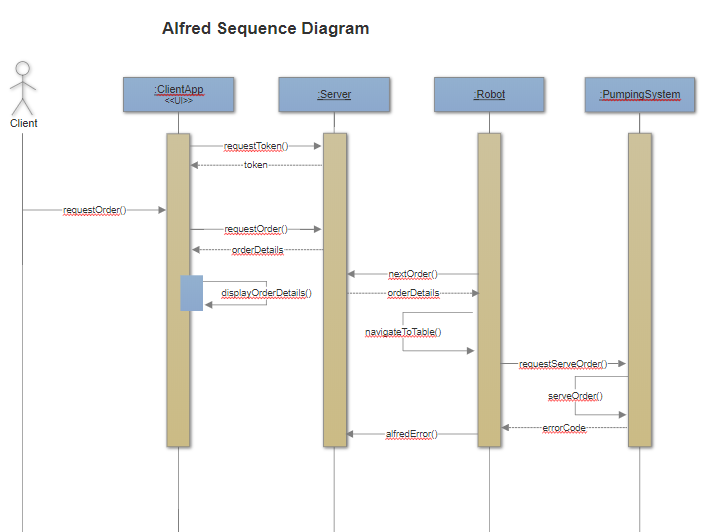
\includegraphics [scale = 0.4] {figures/Alfred_SequenceDiagram.png}
	\caption{Alfred Sequence Diagram}
\end{figure}
\section {Design Notes}

\section {Data Dictionary}

\section {References}
\end{document}
